%   Filename    : chapter_4.tex 
\chapter{Preliminary Results/System Prototype}

\section{System Architecture}
Using the tools mentioned in Section~\ref{sec:devtools}, our system can be visualized as shown in Figure \ref{fig:architecture}: 
\begin{figure}[h] % 'h' places the figure approximately here in the text
	\centering
	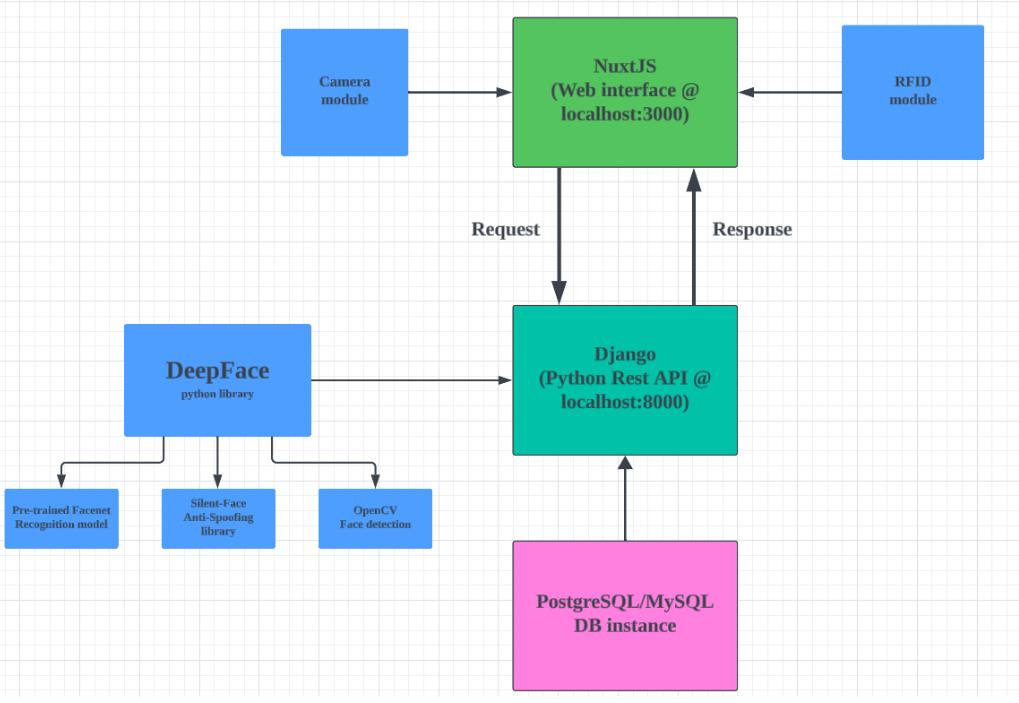
\includegraphics[width=0.8\textwidth]{figures/chapter4/architecture.png} % Adjust width as needed
	\caption{System Architecture}
	\label{fig:architecture}
\end{figure}
\section{Process Diagrams}

\subsection{Faculty CSV Import Process}
	To make the registration of the students much easier for the faculty, the faculty members can upload a CSV file containing the students' required details. The system parses the CSV file and stores the extracted data in the database. The data uploaded is validated to avoid any duplicate or wrong entries.

\subsection{Student Registration Process}
	TODO - Allow student to register themselves

\subsection{Time In Process}
	Time in process includes a check if the student already has time in records. First step in this is the student tapping the ID to the RFID sensor and trigger the photo capture to check the face.
	\begin{figure}[h] % 'h' places the figure approximately here in the text
		\centering
		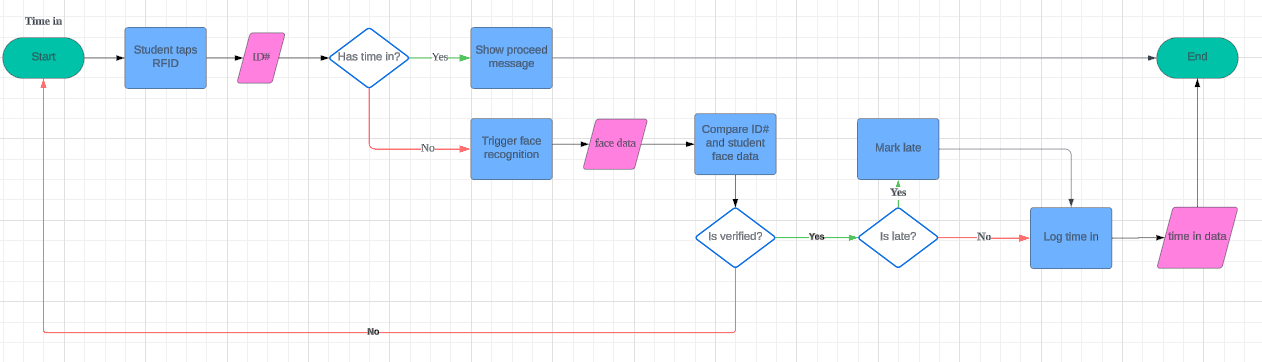
\includegraphics[width=1.0\textwidth]{figures/chapter4/timein.png} % Adjust width as needed
		\caption{Time in}
		\label{fig:timein}
	\end{figure}
	
\subsection{Time Out Process}
\begin{figure}[h] % 'h' places the figure approximately here in the text
	\centering
	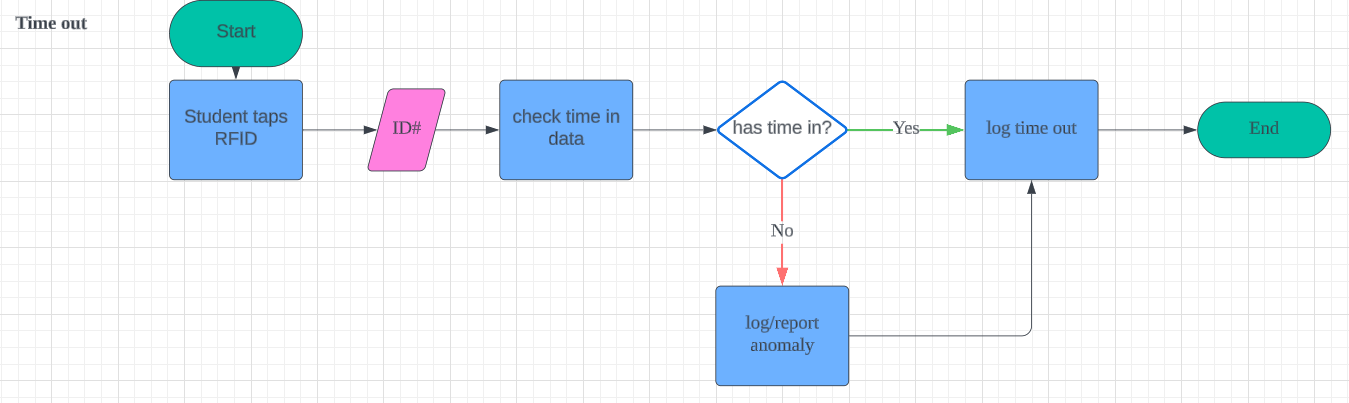
\includegraphics[width=1.0\textwidth]{figures/chapter4/timeout.png} % Adjust width as needed
	\caption{Time Out}
	\label{fig:timeout}
\end{figure}

\subsection{Attendance Record Export Process}
	TODO - Make attendance records exportable as a CSV file

\section{Django Backend}
\subsection{Models}
	Django Model class maps to SQL tables. For example, a Student table will have the following columns which maps to Student Model class' attributes like in Figure \ref{fig:models}: 
	
	\begin{figure}[h] % 'h' places the figure approximately here in the text
		\centering
		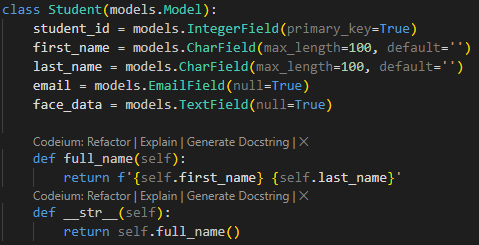
\includegraphics[width=0.8\textwidth]{figures/chapter4/models.png} % Adjust width as needed
		\caption{Student model}
		\label{fig:models}
	\end{figure}
	
	SQL equivalent would be:
	\begin{verbatim}
		CREATE TABLE Student (
		student_id INTEGER PRIMARY KEY,
		first_name VARCHAR(100) NOT NULL DEFAULT '',
		last_name VARCHAR(100) NOT NULL DEFAULT '',
		email VARCHAR(254),
		face_data TEXT,
		CONSTRAINT unique_email UNIQUE (email)
		);
	\end{verbatim}
\subsection{Database Tables}
	Our database tables that can be accessed by Django's ORM. This includes the tables for Teachers, Subjects and tables for relationships. See Figure
	\ref{fig:dbtables}
	\begin{figure}[h] % 'h' places the figure approximately here in the text
		\centering
		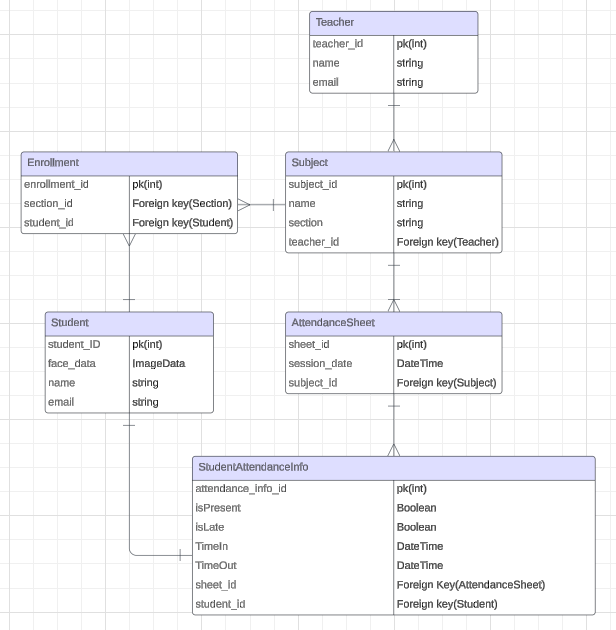
\includegraphics[width=0.8\textwidth]{figures/chapter4/dbtables.png} % Adjust width as needed
		\caption{Database Tables}
		\label{fig:dbtables}
	\end{figure}	
	
\subsection{REST API by Django Ninja}
Figure~\ref{fig:api} is the automatic OpenAPI compliant documentation provided by Django Ninja. It contains all endpoints we can use to query data from the database. All endpoints are protected using HTTP Bearer token authentication.
\begin{figure}[h] % 'h' places the figure approximately here in the text
	\centering
	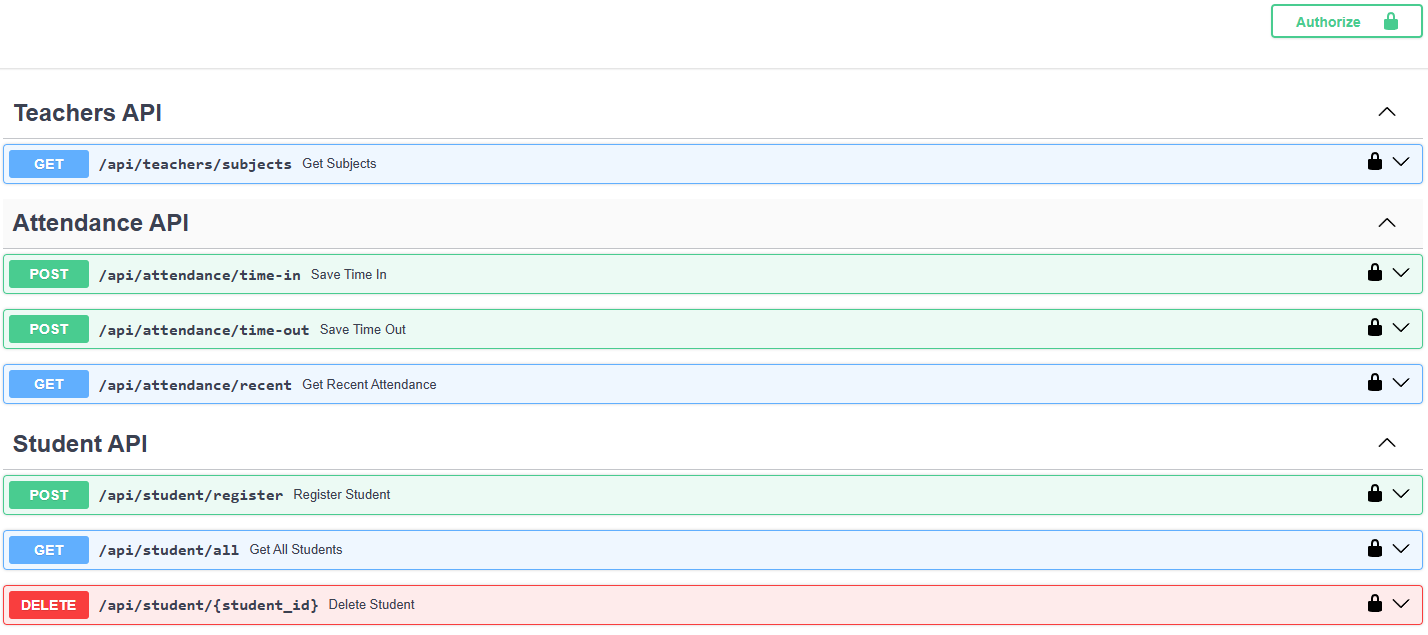
\includegraphics[width=1\textwidth]{figures/chapter4/api.png} % Adjust width as needed
	\caption{API Documentation}
	\label{fig:api}
\end{figure}

\subsection{Admin panel by Django}
Figure~\ref{fig:admin} is the Django administration page only accessible to a superuser account. This is where most of the backend maintanance work happens. It contains all the data inside the database allow full control over them. It also contains every authentication tokens used by each teacher account.
\begin{figure}[h] % 'h' places the figure approximately here in the text
	\centering
	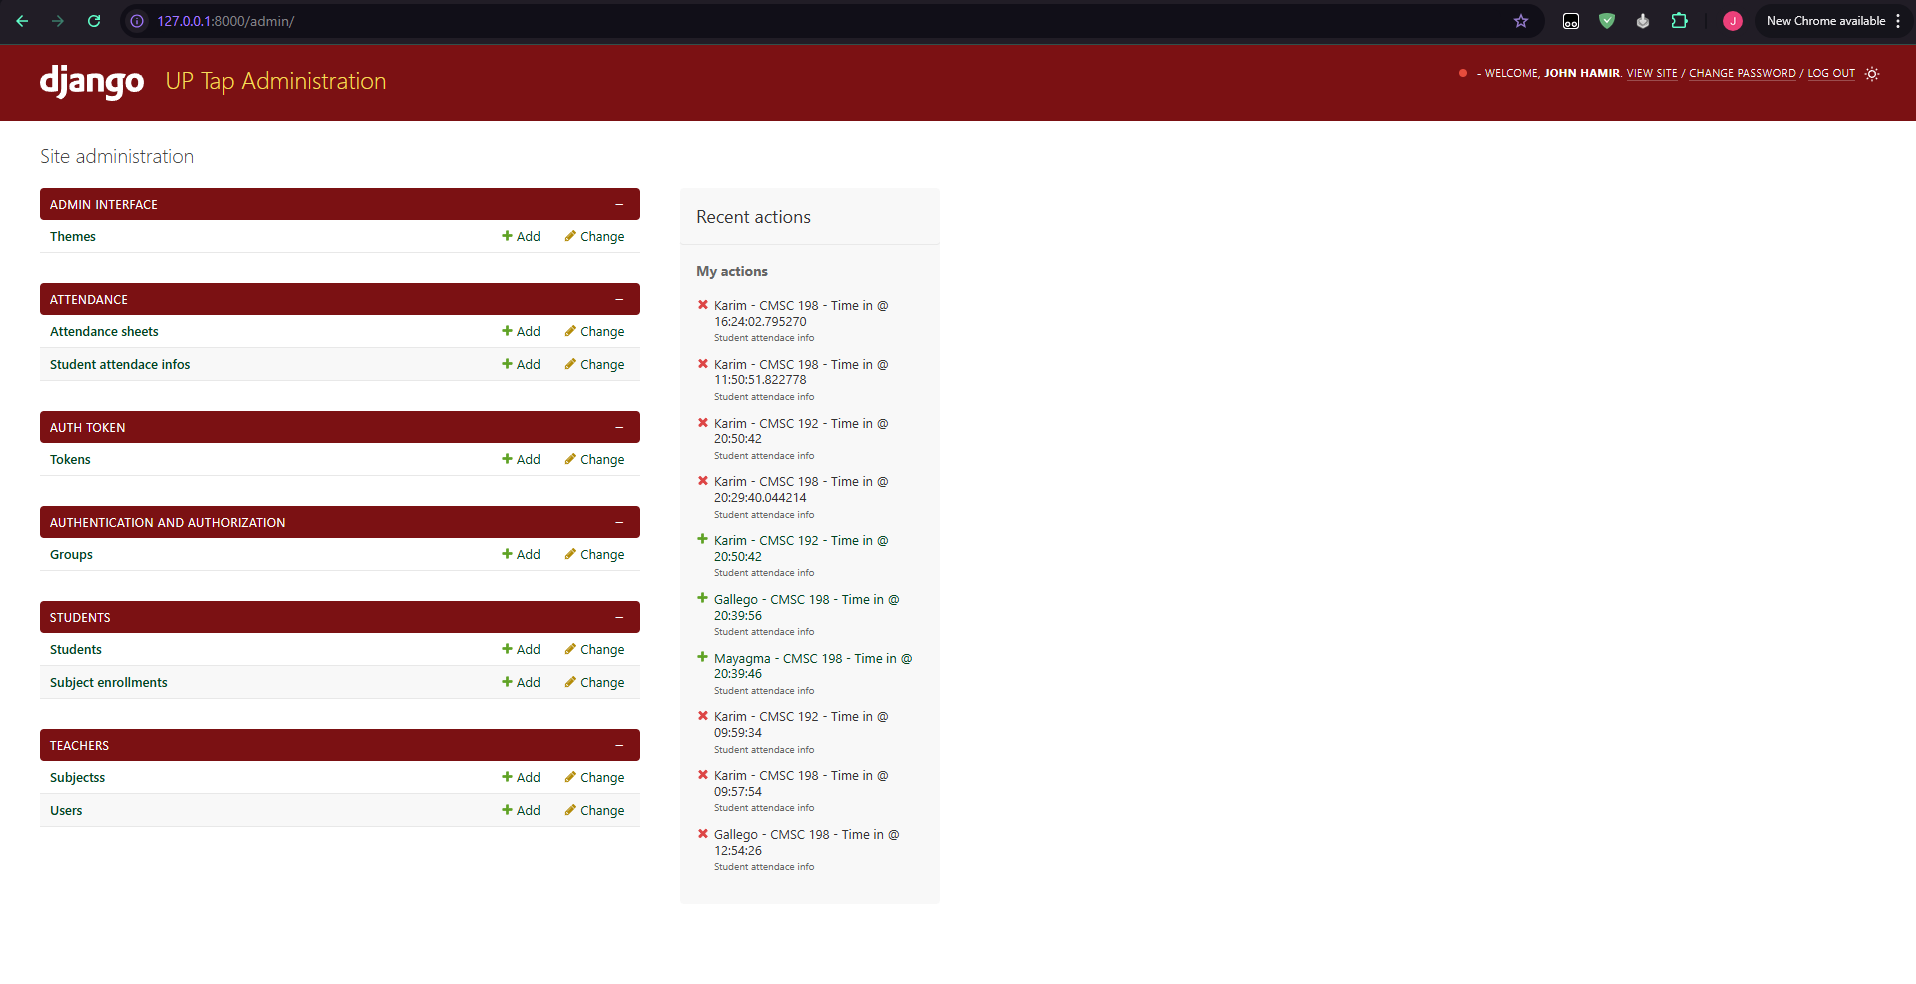
\includegraphics[width=1\textwidth]{figures/chapter4/admin.png} % Adjust width as needed
	\caption{Django Administration}
	\label{fig:admin}
\end{figure}

\section{Nuxt Frontend}
With the backend handling most of the heavy work, the frontend only needs to capture images from the camera and sending them to the backend to verify student identity. The localhost:3000/dashboard/time-in-out page handles the time in and time out process.
\begin{figure}[h] % 'h' places the figure approximately here in the text
	\centering
	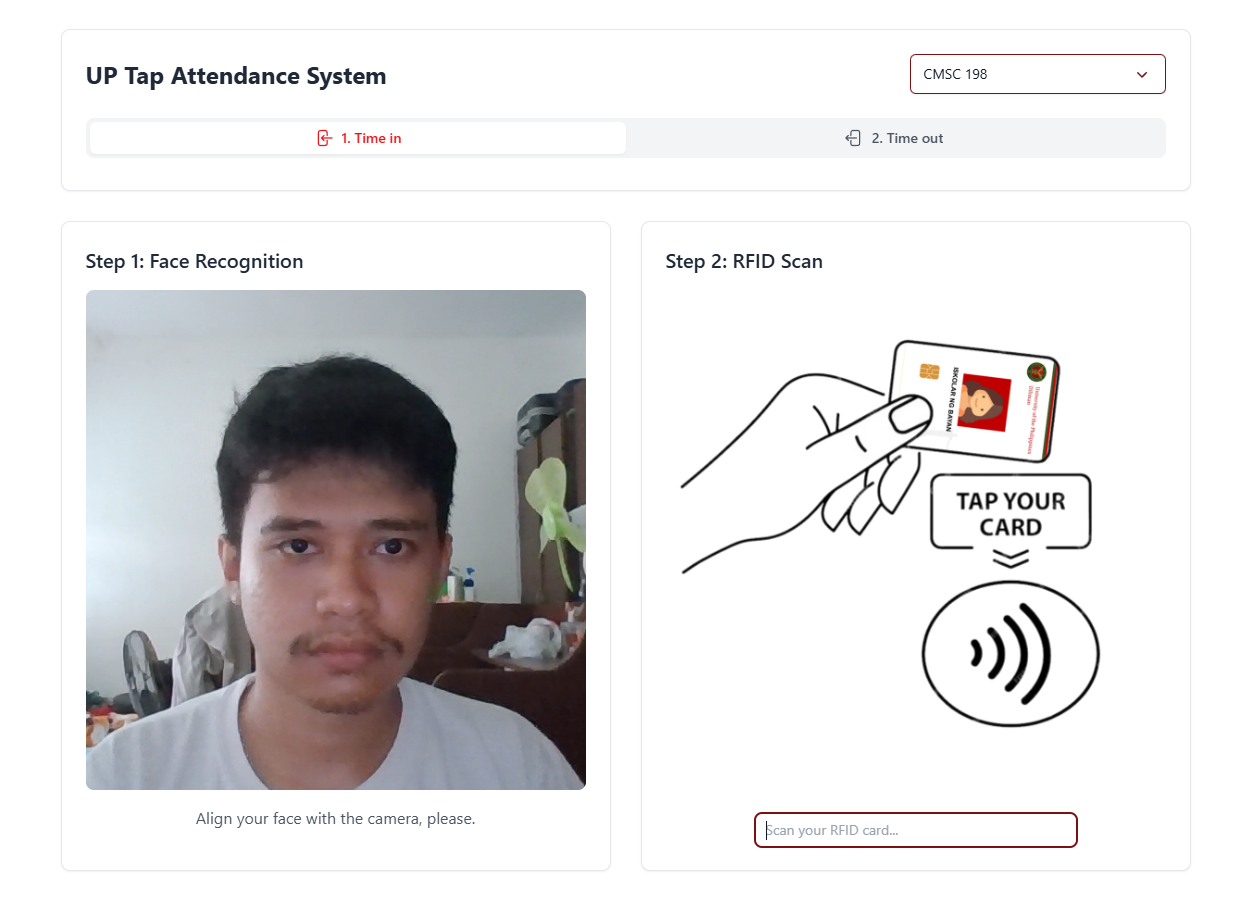
\includegraphics[width=1.0\textwidth]{figures/chapter4/frontend.png} % Adjust width as needed
	\caption{Time in and Time out Page}
	\label{fig:frontend}
\end{figure}
The RFID input is automatically highlighted upon opening the page so it will be immediately ready to take in input from the RFID scanner. When the proper number length is inputted, it will immediately start to verify the identity. It will then notify the student for the time in/time out time and status. It will also notify for any errors like spoof image or no face detected. From our testing, the response time is currently at most 2.3 seconds, most of the delay comes from the fake delay we used to allow the student to read the notification after verification.
\begin{figure}[h] % 'h' places the figure approximately here in the text
	\centering
	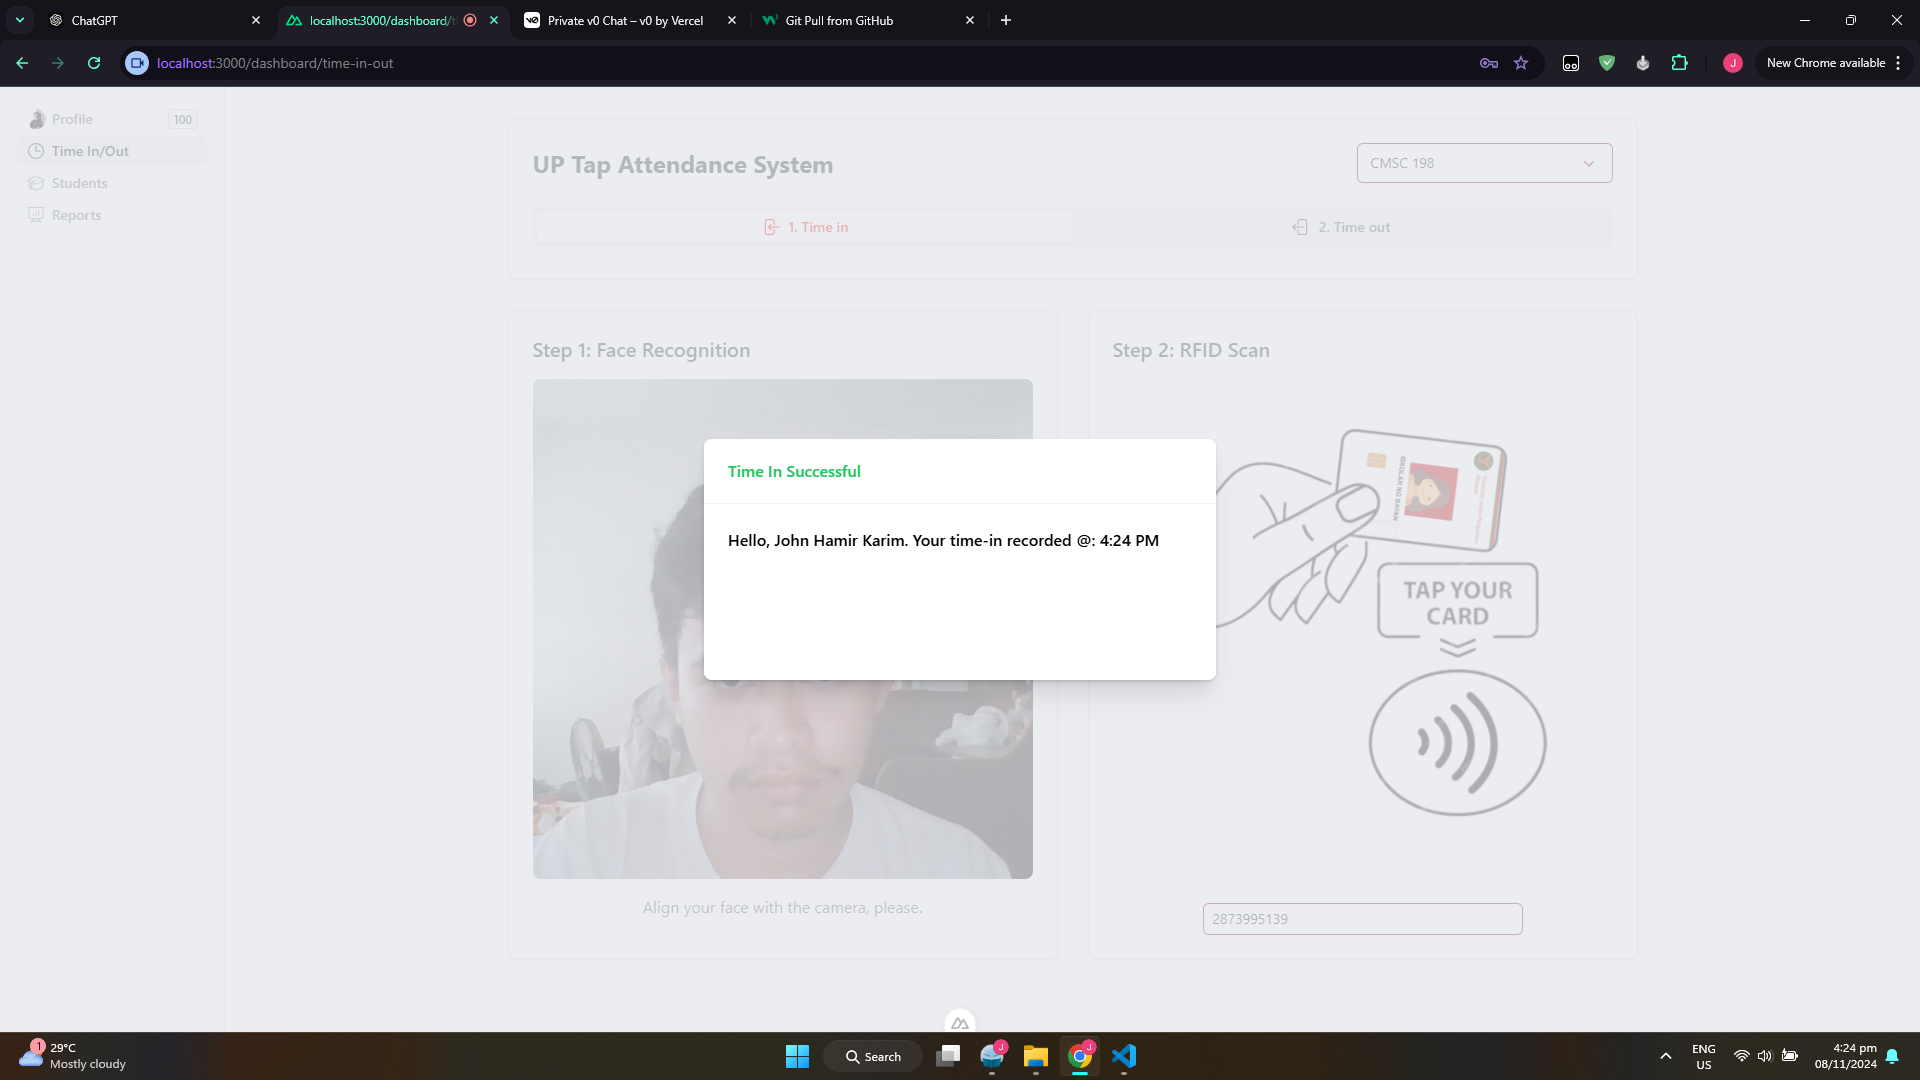
\includegraphics[width=1.0\textwidth]{figures/chapter4/success.png} % Adjust width as needed
	\caption{Successful Time In}
	\label{fig:success}
\end{figure}
\begin{figure}[h] % 'h' places the figure approximately here in the text
	\centering
	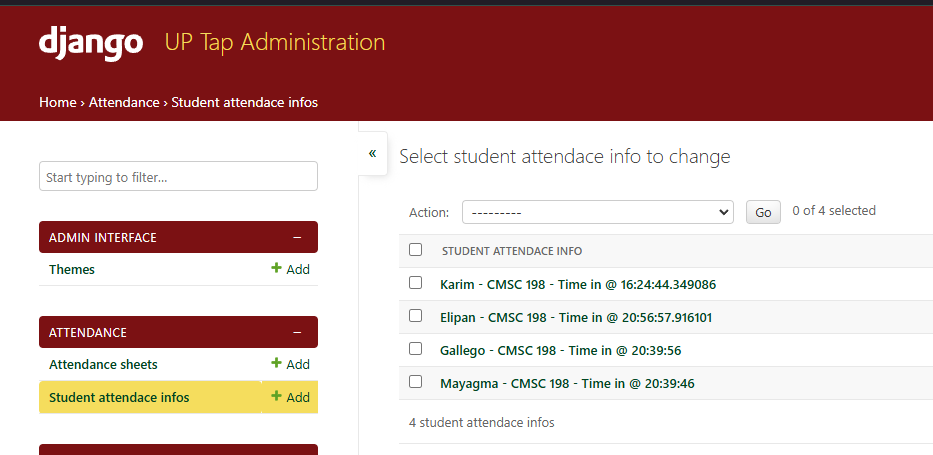
\includegraphics[width=1.0\textwidth]{figures/chapter4/backendrecord.png} % Adjust width as needed
	\caption{Django saving the attendance time instance in 24-hr format}
	\label{fig:record}
\end{figure}
\begin{figure}[h] % 'h' places the figure approximately here in the text
	\centering
	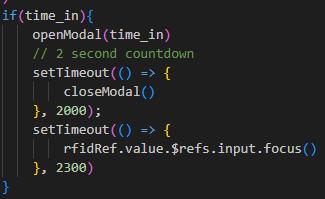
\includegraphics[width=1.0\textwidth]{figures/chapter4/delay.png} % Adjust width as needed
	\caption{Fake Delay}
	\label{fig:delay}
\end{figure}



